% Included in tool.tex
\subsection{Direct Manipulation Gesture Set}

\begin{table}[!b]
% % increase table row spacing, adjust to taste
\renewcommand{\arraystretch}{1.75}
% if using array.sty, it might be a good idea to tweak the value of
% \extrarowheight as needed to properly center the text within the cells
% \setlength{\extrarowheight}{10pt}
\caption{CodeInk's Direct Manipulation Language}
\label{tbl:language_table}
\centering
% % Some packages, such as MDW tools, offer better commands for making tables %
% than the plain LaTeX2e tabular which is used here.
\begin{tabular}{|p{3.8cm} |p{3.8cm} |}
\hline
\textbf{Program Behavior} & \textbf{DM Gesture} \\
\hline
%Access a value & Grab value and drag elsewhere \\
%\hline
Use or copy an object's value & {\em drag-away}: Grab an object, and drag it
away quickly.
Drop it on the canvas to create a new number with the same value.
\\
\hline
Remove an object from its parent (e.g. element from list, node from tree/graph) & {\em dwell-drag-away}: Grab an object, dwell for one second, then
drag it elsewhere.
\\
\hline
Compare two objects' values & {\em drag-into}: Drag one value into another.
\\
\hline
Assign one object's value to another &
{\em drag-into-dwell}: Drag one value into another, and
dwell until the desired interpretation (\texttt{=, +=, -=}) appears. \\
\hline
Insert a value into a list, or a node into a tree/graph
& {\em drag-insert}: Drag the value into a gap in the list, or the node to the
tip of an edge
\\

\hline
Attach an edge to a graph node
& {\em drag-edge}: Drag the edge's start or end handle to the node.
\\

\hline
Mark a list element or tree/graph node (e.g. as sorted or visited) &
{\em fill}: Select the ``Fill" tool, and click on the element. \\
\hline
\end{tabular}
\end{table}

CodeInk's DM gesture set (summarized in Table \ref{tbl:language_table}) enables
users to trace algorithms by manipulating numbers, lists, binary trees and
graphs. From our exercise in watching lecture videos of an introductory
algorithms class, we compiled a list of program behaviors that need to be
expressed when tracing commonly taught sorting and search algorithms (left
column). We then devised a gesture, in keeping with principles of direct
manipulation~\cite{Shneiderman1982, Lee2012}, that would enable the user to
express each behavior using a physical action; for example, numbers can be
copied by grabbing them and dragging away, and they can be inserted into lists
by dragging them into gaps between other elements.

All data structures in CodeInk's visual vocabulary are composed of one or more
objects (list elements or nodes), each with numeric values. For that reason, the
gesture set is both compact (7 in total) and expressive: dragging one object
into another compares their numeric values, regardless of whether they are
numbers, list elements, nodes or some mixture thereof. Similarly, popping a list
element or detaching a subtree from its parent is accomplished by grabbing it
and holding it (\emph{dwelling}) until it can be moved away freely. We will
explain the design decision of introducing dwelling later.

% The gesture set is best explained through examples, which we provide below.

\subsection{Worked Example: Insertion Sort}
Tracing insertion sort's execution on an example list is usually performed by
storyboarding its behavior, redrawing the list in several new configurations
(\fig{fig:6006-insertion}). In CodeInk, the algorithm can be traced as follows:

\noindent 1) Drag an example list onto the canvas and type in a comma-separated
set of numbers to initialize its values (green arrows indicate drag motion and
are not part of the CodeInk UI).

\vspace{-0.25em}
\noindent 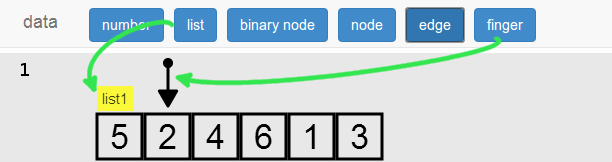
\includegraphics[width=0.7\columnwidth]{img/examples/insertion-1.png}
\vspace{0.5em}

\noindent 2) To prepare to move the ``2" element, grab and hold the element for
at least one second (\emph{dwell}). A blue circle fills up to give the user
feedback on how long they have dwelled.

\vspace{-0.25em}
\noindent 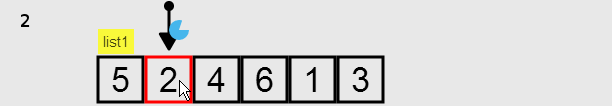
\includegraphics[width=0.7\columnwidth]{img/examples/insertion-2.png}
\vspace{0.4em}

\noindent 3) After one second has elapsed (blue circle filled entirely), the
list expands outward, creating gaps into which the element can be inserted. The
``2" element is ready to be moved.

\vspace{-0.25em}
\noindent 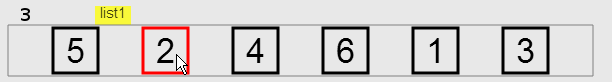
\includegraphics[width=0.7\columnwidth]{img/examples/insertion-3.png}
\vspace{0.5em}

\noindent 4) Drag the ``2" to the left until it hits the ``5" element, which
creates a numeric comparison step (``2 $<$ 5") in the trace.

\vspace{-0.25em}
\noindent 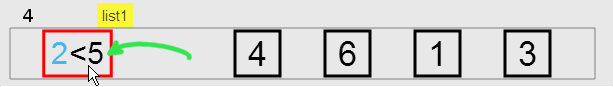
\includegraphics[width=0.7\columnwidth]{img/examples/insertion-4.png}
\vspace{0.5em}

\noindent 5) Keep moving the ``2" to the left of the ``5" element.

\vspace{-0.25em}
\noindent 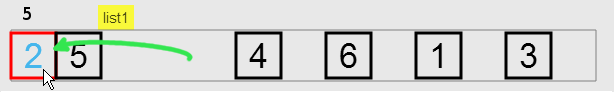
\includegraphics[width=0.7\columnwidth]{img/examples/insertion-5.png}
\vspace{0.5em}

\noindent 6) Once the correct position is found, drop the element
to create a list insertion step in the trace. The list collapses again in its new, rearranged state, with the
``2" preceeding the ``5''.

\noindent 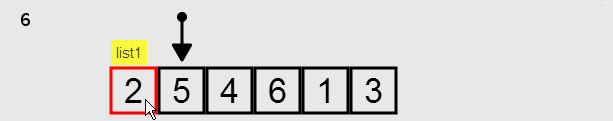
\includegraphics[width=0.7\columnwidth]{img/examples/insertion-6.png}

The user explains the rest of insertion sort by moving down the list and
inserting elements into the sorted sublist until the entire list is sorted. If
any mistakes are made, the user can \emph{undo} steps to remove them from the
trace. Many list sorting and searching algorithms can be explained using this
subset of CodeInk's direct manipulation language: creating lists and dragging
elements to show comparisons and rearrangements.

\subsection{Example: AVL Insertion}
Tracing an AVL (balanced binary search tree) insertion can be a tedious and
error-prone process, because rotations have to be shown by redrawing the
entire tree in a new configuration. CodeInk's gesture set affords users the
ability to rearrange nodes in the tree by detaching, dragging and reattaching
them.

\noindent \begin{tabular}{m{4.6cm} m{3.4cm}}

1) Create two new binary tree nodes (``4" and ``6") by dragging node
objects onto the canvas and typing in their values.

& 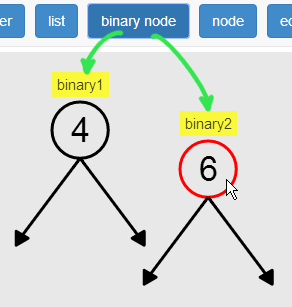
\includegraphics[width=3.4cm]{img/examples/bst-1.png}
\end{tabular}


\noindent \begin{tabular}{m{4.6cm} m{3.4cm}}

2) Drag the ``6'' node into the ``4'' node to compare their values.
CodeInk adds the comparison step (``4 $<$ 6") to the trace.

& 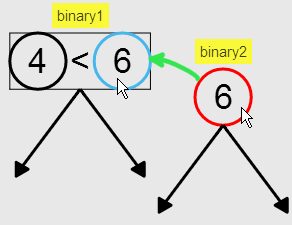
\includegraphics[width=3.4cm]{img/examples/bst-2.png}
\end{tabular}

\noindent \begin{tabular}{m{6.2cm} m{1.8cm}}

3) Since ``6" is greater than ``4", keep dragging the ``6'' along the
right pointer of the ``4" node. This temporarily highlights the pointer
blue and adds a \emph{pointer traversal} step to the trace.

& 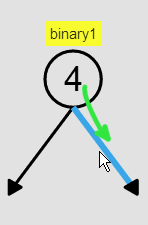
\includegraphics[width=1.8cm]{img/examples/bst-3.png}
\end{tabular}

\noindent \begin{tabular}{m{4.6cm} m{3.4cm}}

4) Keep dragging along the right pointer until reaching its tip. The
``6" node now re-emerges as the right child of ``4." The node is colored blue to
preview the insertion. Release the node to confirm the insertion:
\texttt{binary1.right = binary2}

& 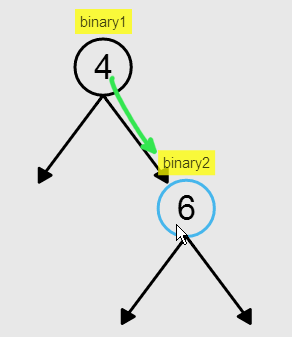
\includegraphics[width=3.4cm]{img/examples/bst-4.png}
\end{tabular}

\noindent \begin{tabular}{m{4.6cm} m{3.4cm}}

5) Next insert a new ``9" node into the tree, which results in an
unbalanced tree. Now demonstrate a rotation by grabbing the ``6" node,
dwelling for one second, and dragging it away to detach the subtree.
When the subtree is dropped on the canvas, a new step is added to the
trace: \texttt{binary1.right = None}

& 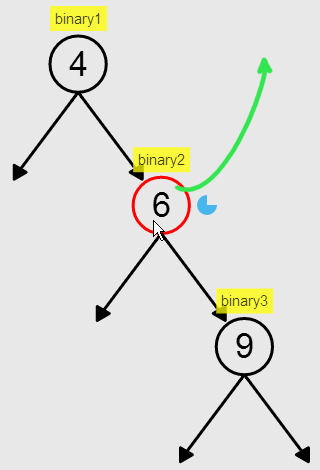
\includegraphics[width=3.4cm]{img/examples/bst-5.png}
\end{tabular}

\noindent \begin{tabular}{m{4.6cm} m{3.4cm}}

6) The ``6 / 9" subtree is now separated from the ``4." Drag the ``4"
node downward ...

& 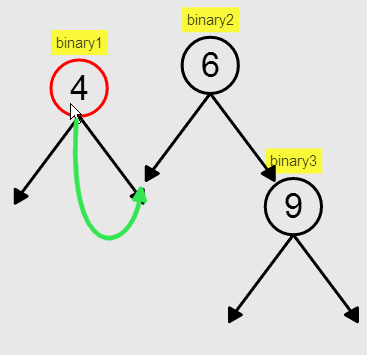
\includegraphics[width=3.4cm]{img/examples/bst-6.png}
\end{tabular}

\noindent \begin{tabular}{m{4.6cm} m{3.4cm}}

7) ... until it reaches the tip of the ``6" node's left pointer, then
release to insert it there and balance the tree: \texttt{binary2.left =
binary1}

& 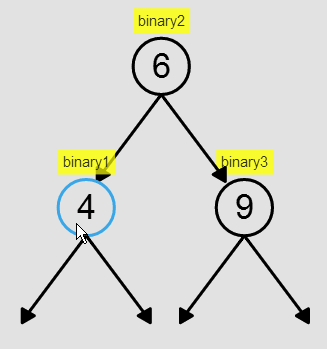
\includegraphics[width=3.4cm]{img/examples/bst-7.png}
\end{tabular}

As is the case with lists, dragging one value into another triggers a
numeric comparison (step 2), and grabbing and dwelling on a child object
removes it from its parent data structure (step 5).

\begin{comment}
\noindent \textbf{Graph algorithms}: Our language also covers graph
traversal, such as search or finding shortest paths (see
\fig{fig:example-dijkstra}). It supports creating and attaching graph
nodes and edges, updating node and edge values, and marking nodes as
visited. Here is how to trace Dijkstra's algorithm using CodeInk:

\noindent \begin{tabular}{m{4.2cm} m{3.8cm}}
1) Create an example graph by dragging and dropping node and edge
objects onto the canvas, typing in the numeric node costs and edge weights.
Edges can be connected to nodes by clicking and dragging their start and end
handles.
& 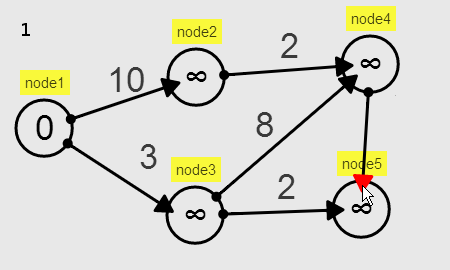
\includegraphics[width=3.8cm]{img/examples/dijkstra-1.png}
\end{tabular}

\noindent \begin{tabular}{m{4.2cm} m{3.8cm}}
2) Start with \texttt{node1}. To calculate the
cost of reaching its neighbor \texttt{node2},
first drag \texttt{node1} (source node) and drop it onto the canvas, which
creates a new number (\texttt{num1}) equal to the node's cost (\texttt{0}).
& 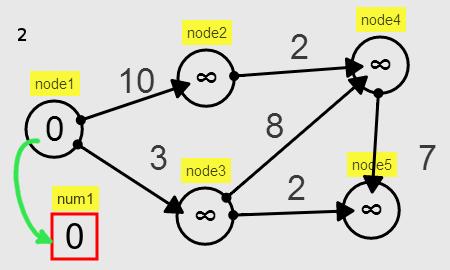
\includegraphics[width=3.8cm]{img/examples/dijkstra-2.png}
\end{tabular}

\noindent \begin{tabular}{m{4.2cm} m{3.8cm}}
3) Now drag the weight of the connecting edge into the current cost
(\texttt{num1}), which triggers a comparison by default. However, a
comparison is not the correct operation; the two values
must be added.
& 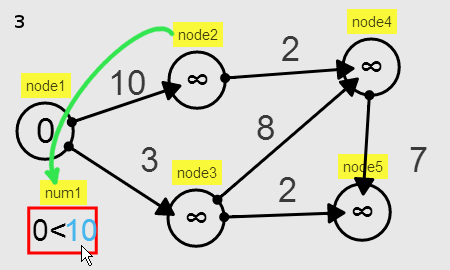
\includegraphics[width=3.8cm]{img/examples/dijkstra-3.png}
\end{tabular}

\noindent \begin{tabular}{m{4.2cm} m{3.8cm}}
4) Dwelling after the drag-into gesture causes CodeInk to cycle through alternative
interpretations. When an addition assignment
operation (\texttt{+=}) appears, release to end the gesture. The cost
updates to the value of \texttt{10} (\texttt{num1 += edge1.weight}).
& 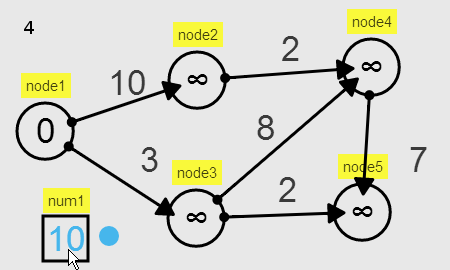
\includegraphics[width=3.8cm]{img/examples/dijkstra-4.png}
\end{tabular}

\noindent \begin{tabular}{m{4.2cm} m{3.8cm}}
5) Now drag \texttt{num1} into \texttt{node2}
to trigger a comparison, checking if the new cost is less than
the existing cost of reaching that node.
& 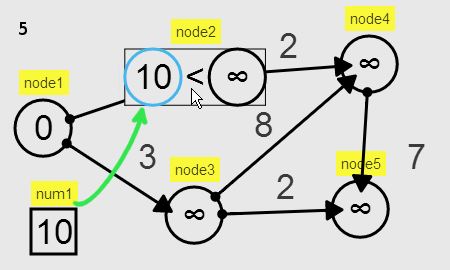
\includegraphics[width=3.8cm]{img/examples/dijkstra-5.png}
\end{tabular}

\noindent \begin{tabular}{m{4.2cm} m{3.8cm}}
6) Since \texttt{10 $<$ $\infty$}, dwell to cycle to the assignment
expression (\texttt{node2.value = num1}). Releasing ends the gesture, and updates the cost
of \texttt{node2} to 10.
& 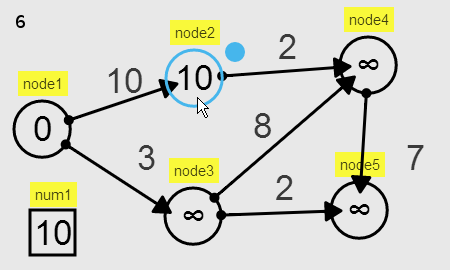
\includegraphics[width=3.8cm]{img/examples/dijkstra-6.png}
\end{tabular}

\noindent \begin{tabular}{m{4.2cm} m{3.8cm}}
7) Repeat on all nodes and mark each one as visited by
selecting ``Fill" and clicking on that node.
& 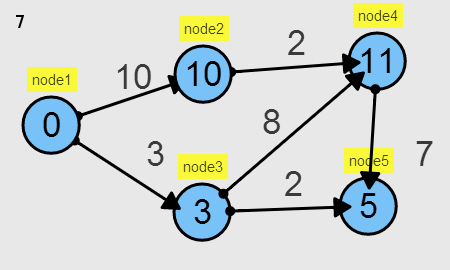
\includegraphics[width=3.8cm]{img/examples/dijkstra-7.png}
\end{tabular}

%Because the drag-into gesture has multiple interpretations
%(comparison, assignment, addition assignment), the user can dwell
%to cycle through all interpretations (see \sec{sec:overloaded-gestures}).
\end{comment}

\subsection{Chaining and traversal patterns}
The user can chain multiple gestures while dragging an object. One common
example of chaining arises when describing a traversal pattern involving a
series of comparisons. For example, during insertion sort, the user can drag an
element along the list, performing comparisons without releasing it until the
correct location is found. When the location is found, the user can release the
element into the gap between two existing elements, resulting in an insertion.

One subtle interaction issue during a chain of gestures is deciding which
behaviors to commit to the list of steps, and which to omit. For example, the
user should be allowed to drag an element into a list, then undo the behavior by
dragging it back out of the list. The insertion should be committed only when
the new value is released into the list. However, other behaviors like
comparisons should be committed while the user continues to drag, since they are
performed as part of the traversal pattern. Note that in the insertion sort
demonstration, there is only one grab, drag, and release, but both the
numeric comparison and swap are added to the trace. The same applies for
the AVL insertion, where the candidate node is dragged
through the tree in one motion, until it is released at a leaf.

In exploring this issue of which behaviors to commit, we have found it useful to
distinguish between mutation and observation behaviors. Mutation behaviors are
those that result in data structure changes (e.g., insertions, assignments), while
observation behaviors only visualize decision making in the algorithm
(e.g., comparisons, following pointers), and do not affect the underlying data
structures. In a chain of gestures, observation behaviors are continuously
committed to the algorithm's trace, while mutation behaviors are committed
only if the data structure has changed at the end of a gesture.

\subsection{Resolving overloaded gestures}
\label{sec:overloaded-gestures}

When designing a gesture vocabulary, the gesture that seems most natural for a
task can often be interpreted in multiple ways. There are two main examples of
this in CodeInk's language: ambiguity in the drag-into gesture, and ambiguity in
the drag-away gesture when the value is part of some higher-level data structure
(e.g. a list element, or a child node in a tree or graph).

The drag-into gesture is ambiguous because dragging one object into
another could be interpreted as a comparison (\texttt{x$<$y}), an
assignment (\texttt{x=y}), or an augmented assignment such as
\texttt{x+=y} or \texttt{x-=y}.

Performing the drag-away gesture on a child object is ambiguous because it is
not obvious whether the parent object should be altered or not. For example,
when dragging an element away from a list, should a copy of the element be made,
or should the element be pulled out of the parent list? For trees and graphs,
should a copy of the dragged node be made, or should that node and its
descendants be detached from the parent?

Our solution is to default to the observation behavior of a gesture, and preview
other possible mutation behaviors if the user dwells for more than one second.
This means defaulting to a comparison for the drag-into gesture, and making a
copy of the dragged value for the drag-away gesture.
%
This is also useful for a chained traversal pattern, since the comparisons
can occur in quick succession while dragging without dwelling.

%In order to make an assignment, the user can drag the source object into
%the target and dwell. At that point, the system cycles through different
%interpretations of the gesture. In the case of dragging a child object,
%the user selects and dwells on a list element or node until it turns
%blue, indicating it has been detached from its parent.
